\documentclass{exam}
\usepackage[utf8]{inputenc}
\usepackage{lmodern}
\usepackage{microtype}

% \usepackage[parfill]{parskip}
\usepackage[dvipsnames]{xcolor}
\usepackage{amsmath}
\usepackage{amsfonts}
\usepackage{amsthm}
\usepackage{siunitx}
\DeclareSIUnit\year{yr}
\DeclareSIUnit\foot{ft}
\DeclareSIUnit\litre{\liter}

\usepackage{skull}

\usepackage{pgfplots}
\usepgfplotslibrary{polar}
\pgfplotsset{compat=1.11}
\usepgfplotslibrary{statistics}
\usepackage{graphicx}
\usepackage{sidecap}
\sidecaptionvpos{figure}{c}
\usepackage{float}
\usepackage{gensymb}
\usepackage{tkz-euclide}
\usetkzobj{all}
\usepackage{commath}
\usepackage{hyperref}
\usepackage{enumitem}
\usepackage{wasysym}
\usepackage{multicol}
\usepackage{mathtools}
\usepackage{tcolorbox}
\usepackage{tabularx}
\usepackage[version=4]{mhchem}
\usepackage{changepage}
\usepackage{listings}
\lstset{basicstyle=\ttfamily\linespread{0.8}\small}

\renewcommand*{\thefootnote}{\fnsymbol{footnote}}

\newtheorem*{thm}{Theorem}
\newtheorem*{iden}{Identity}
\newtheorem*{lemma}{Lemma}
\newtheorem{obs}{Observation}
\theoremstyle{definition}
\newtheorem*{defn}{Definition}
\newtheorem*{ex}{Example}
\newtheorem{con}{Construction}
\newtheorem*{alg}{Algorithm}

\newtheoremstyle{break}
  {\topsep}{\topsep}%
  {\itshape}{}%
  {\bfseries}{}%
  {\newline}{}%
\theoremstyle{break}
\newtheorem*{bthm}{Theorem}

% russian integral
\usepackage{scalerel}
\DeclareMathOperator*{\rint}{\scalerel*{\rotatebox{17}{$\!\int\!$}}{\int}}

% \DeclareMathOperator*{\rint}{\int}

\pgfplotsset{vasymptote/.style={
    before end axis/.append code={
        \draw[densely dashed] ({rel axis cs:0,0} -| {axis cs:#1,0})
        -- ({rel axis cs:0,1} -| {axis cs:#1,0});
    }
}}

% \pointsinrightmargin
\boxedpoints
\pointname{}

\newcommand{\questioA}{\question[\texttt{\textbf{\color{Cerulean} A}}]}
\newcommand{\questioM}{\question[\texttt{\textbf{\color{PineGreen} M}}]}
\newcommand{\questioE}{\question[\texttt{\textbf{\color{WildStrawberry} E}}]}
\newcommand{\questioS}{\question[\texttt{\textbf{\color{Goldenrod} S}}]}
\newcommand{\questioO}{\question[\texttt{\textbf{\color{BurntOrange} O}}]}

\newcommand{\parA}{\part[\texttt{\textbf{\color{Cerulean} A}}]}
\newcommand{\parM}{\part[\texttt{\textbf{\color{PineGreen} M}}]}
\newcommand{\parE}{\part[\texttt{\textbf{\color{WildStrawberry} E}}]}
\newcommand{\parS}{\part[\texttt{\textbf{\color{Goldenrod} S}}]}
\newcommand{\parO}{\part[\texttt{\textbf{\color{BurntOrange} O}}]}

\newcommand{\subparA}{\subpart[\texttt{\textbf{\color{Cerulean} A}}]}
\newcommand{\subparM}{\subpart[\texttt{\textbf{\color{PineGreen} M}}]}
\newcommand{\subparE}{\subpart[\texttt{\textbf{\color{WildStrawberry} E}}]}
\newcommand{\subparS}{\subpart[\texttt{\textbf{\color{Goldenrod} S}}]}
\newcommand{\subparO}{\subpart[\texttt{\textbf{\color{BurntOrange} O}}]}

\newcommand{\mainHeader}[2]{\section*{NCEA Level 2 Mathematics\\#1. #2}}
\newcommand{\mainHeaderHw}[2]{\section*{NCEA Level 2 Mathematics (Homework)\\#1. #2}}
\newcommand{\seealso}[1]{\begin{center}\emph{See also #1.}\end{center}}
\newcommand{\drills}[1]{\begin{center}\emph{Drill problems: #1.}\end{center}}
\newcommand{\basedon}[1]{\begin{center}\emph{Notes largely based on #1.}\end{center}}


\begin{document}

\mainHeader{3}{Trigonometry}
\begin{center}
  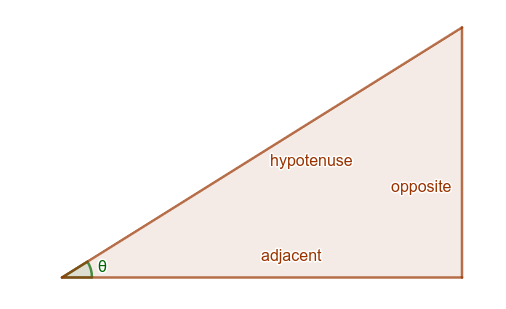
\includegraphics[width=0.5\textwidth]{trig}
\end{center}
We are now going to look at triangles inside circles. Now, last year we learned that any triangles with two equal angles are similar; in particular,
if we take ratios of sides, we obtain the same value. This means that if we have any right-angled triangle with angle $ \theta $ like the one above,
then the ratios $ \frac{\text{opposite}}{\text{hypotenuse}} $, $ \frac{\text{adjacent}}{\text{hypotenuse}} $, and $ \frac{\text{opposite}}{\text{adjacent}} $
all depend only on the angle $ \theta $; we call them the sine, cosine, and tangent of the angle respectively:
\begin{displaymath}
  \sin \theta = \frac{\text{opposite}}{\text{hypotenuse}}\qquad \cos \theta = \frac{\text{adjacent}}{\text{hypotenuse}} \qquad \tan \theta = \frac{\text{opposite}}{\text{adjacent}} = \frac{\sin\theta}{\cos\theta}.
\end{displaymath}

In particular, if we draw our triangle inside a unit circle then we can draw the following:
\begin{center}
  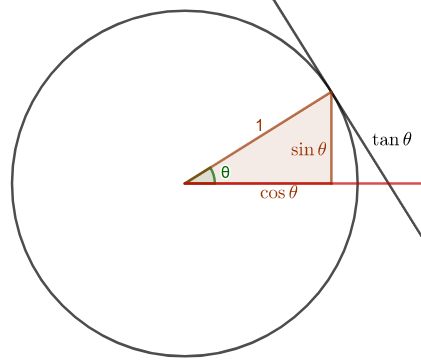
\includegraphics[width=0.4\textwidth]{trigfns}
\end{center}
In fact, we can take this as our definition of $ \sin $ and $ \cos $. To show that $ \tan \theta $ is indeed the line segment marked there,
first notice that since the large triangle is right-angled, the angle at the intersection of the horizontal line and the tangent line
is $ \ang{90} - \theta $; so the other non-right-angle in the smaller triangle is $ \theta $. Hence the hypotenuse of the triangle
is $ \frac{\text{adjacent}}{\cos \theta} = \frac{\sin\theta}{\cos\theta} $, as proposed.

Note also that, from this diagram, we have
\begin{displaymath}
  \sin^2 \theta + \cos^2  \theta = 1
\end{displaymath}
for every angle $ \theta $.

Since the $ \sin $ of an angle is just the height of the point above the $ x$-axis in the diagram above, we have that $ -1 \leq \sin \theta \leq 1 $;
similarly, $ -1 \leq \cos \theta \leq 1 $. Note that when $ \theta = \ang{90} $, the tangent line becomes horizontal and so never intersects the $ x$-axis:
so $ \tan \ang{90} $ is undefined. We can even graph $ \sin \theta $ (red), $ \cos \theta $ (blue), and $ \tan \theta $ (green):
\begin{center}
  \fbox{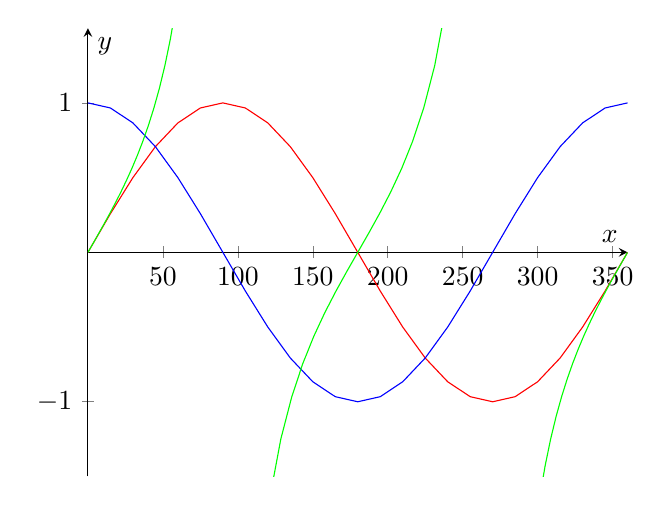
\begin{tikzpicture}
    \begin{axis}[
      axis lines = center,
      ymax = 1.5, ymin = -1.5,
      xlabel = $ x $,
      ylabel = $ y $
    ]
      \addplot[domain = 0:360, color = red] {sin(x)};
      \addplot[domain = 0:360, color = blue] {cos(x)};
      \addplot[domain = 0:88, color = green] {tan(x)};
      \addplot[domain = 92:268, color = green] {tan(x)};
      \addplot[domain = 272:360, color = green] {tan(x)};
    \end{axis}
  \end{tikzpicture}}
\end{center}

If we graph them in radians, only the labels on the $ x$-axis change:
\begin{center}
  \fbox{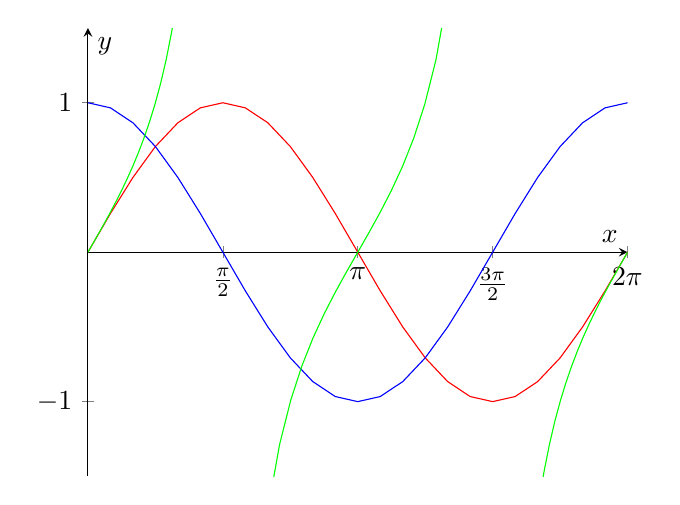
\begin{tikzpicture}
    \begin{axis}[
      axis lines = center,
      ymax = 1.5, ymin = -1.5,
      xtick={1.5708, 3.14159, 4.7124, 6.28},
      xticklabels={$\frac{\pi}{2}$,$\pi$,$\frac{3\pi}{2}$,$2\pi$},
      xlabel = $ x $,
      ylabel = $ y $
    ]
      \addplot[domain = 0:2*pi, color = red] {sin(deg(x))};
      \addplot[domain = 0:2*pi, color = blue] {cos(deg(x))};
      \addplot[domain = 0:(pi/2-0.01), color = green] {tan(deg(x))};
      \addplot[domain = (pi/2+0.01):(3*pi/2-0.01), color = green] {tan(deg(x))};
      \addplot[domain = (3*pi/2+0.01):2*pi, color = green] {tan(deg(x))};
    \end{axis}
  \end{tikzpicture}}
\end{center}

Let us now begin to look at more general triangles:
\begin{center}
  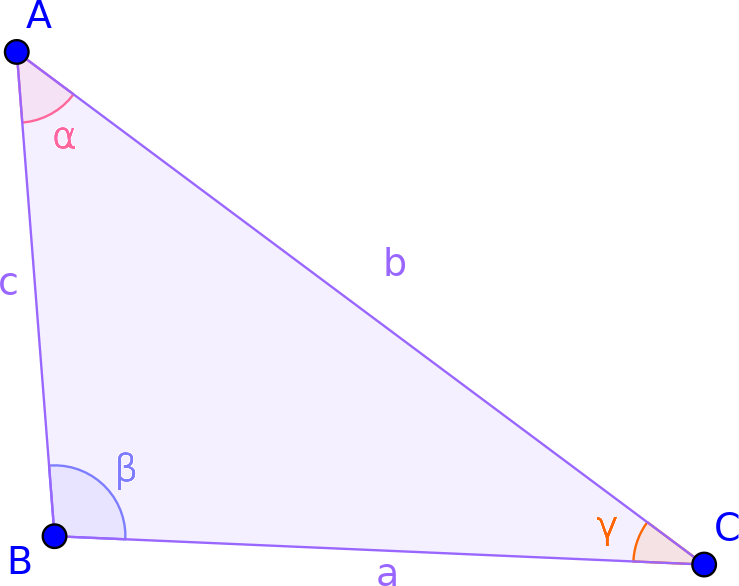
\includegraphics[width=0.3\textwidth]{trisines}
\end{center}

\begin{thm}[Sine rule]
  In any triangle, with the angles and sides labelled as above, we have
  \begin{displaymath}
    \frac{\alpha}{\sin a} = \frac{\beta}{\sin b} = \frac{\gamma}{\sin c}.
  \end{displaymath}
\end{thm}
\begin{proof}
  Drop an altitude from $ B $ to $ AC $, creating two new right-angled triangles. Then the length of this line can be calculated using both
  of the resulting right-angled triangles: so $ c \sin \alpha = a \sin \gamma $ and $ \frac{a}{\sin \alpha} = \frac{c}{\sin \gamma} $. This
  proves the theorem.
\end{proof}

\begin{thm}[Cosine rule]
  In any triangle, with the angles and sides labelled as above, we have
  \begin{displaymath}
    a^2 = b^2 + c^2 - bc\cos \alpha.
  \end{displaymath}
\end{thm}
\begin{proof}
  Drop an altitude from $ B $ to $ AC $, creating two new right-angled triangles. Then the length $ b $ can be split into two
  lengths, $ c \cos \alpha $ and $ b - c \cos \alpha $; the length of the altitude is $ c \sin \alpha $. Now, apply the Pythagorean
  theorem to the triangle including the angle $ \gamma $:
  \begin{displaymath}
    a^2 = (b - c \cos \alpha)^2 + c^2 \sin^2 \alpha = b^2 - 2bc \cos \alpha + c^2 \cos^2 \alpha + c^2 \sin^2 \alpha = b^2 + c^2 - 2bc \cos \alpha.
  \end{displaymath}
\end{proof}

\subsection*{Questions}
\begin{questions}
  \question A beam of gamma rays is to be used to treat a tumor known to be $ \SI{5.7}{\centi\metre} $ beneath
            the patient's skin. To avoid damaging a vital organ, the radiologist moves the source over by
            $ \SI{8.3}{\centi\metre} $.
    \begin{parts}
      \part At what angle to the patient's skin must the radiologist aim the gamma ray source to hit the tumor?
      \part How far will the beam have to travel through the patient's body before reaching the tumor?
    \end{parts}

  \question A surveyor measures the three sides of a triangular field and finds that they are 117, 165, and 257~metres long.
    \begin{parts}
      \part What is the measure of the largest angle of the field?
      \part What is the area of the field?
    \end{parts}

  \question A field has the shape of a quadrilateral (four-sided shape) that is \emph{not} a rectangle. Three
            sides measure 2.33, 3.97, and 3.9~kilometres, and two angles measure $ \alpha = \ang{131.06} $
            and $ \gamma = \ang{86.05} $ (as in the figure).
            \begin{center}
              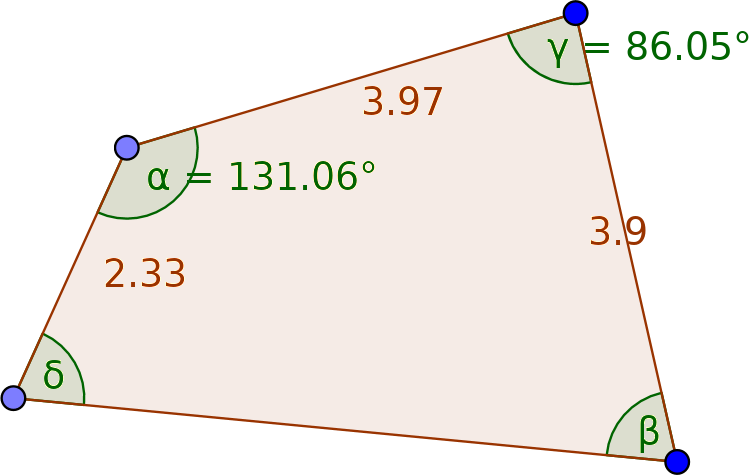
\includegraphics[width=0.3\textwidth]{fieldfortrig}
            \end{center}
    \begin{parts}
      \part By dividing the quadrilateral into two triangles, find its area.
      \part Find the length of the fourth side.
      \part Find the measures of the other two angles, $ \beta $ and $ \delta $.
    \end{parts}

  \question A surveyor is standing on top of a peak. She can see two prominent peaks ahead of her, and from previous measurements
            she knows that one of them is $ \SI{8}{\kilo\metre} $ away from her and the other is $ \SI{11}{\kilo\metre} $ away. She
            measures the angle between them to be $ \ang{120} $. How far apart are the two peaks (measured \emph{along the ground}):
            \begin{parts}
              \part If that they have same height?
              \part If the surveyor and the closer peak are at the same height, but the peak which is further away is \SI{200}{\metre} higher?
            \end{parts}
  \question Consider a triangle with sides of 5, 7, and 10 kilometres.
        \begin{subparts}
          \subpart Find the measure of the largest angle of this triangle.
          \subpart Find the area of the triangle.
        \end{subparts}
    \end{parts}
  \clearpage
  \question Find the area of the triangle below.
            \begin{center}
              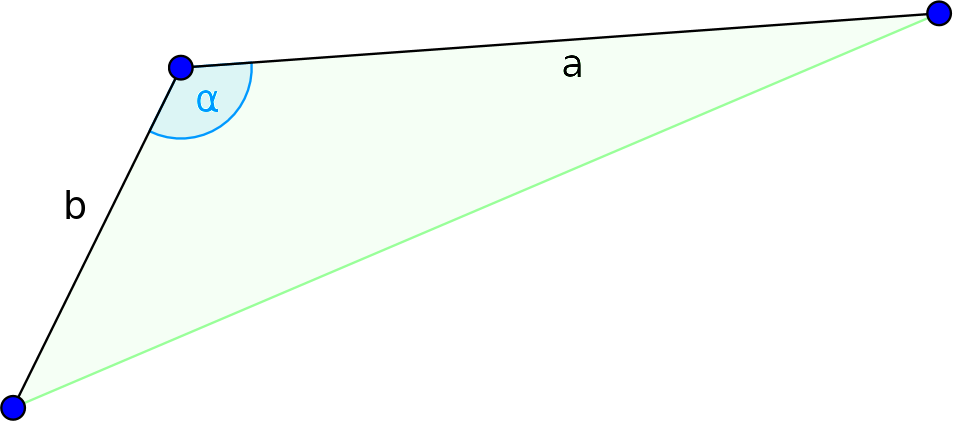
\includegraphics[width=0.3\textwidth]{triarea}
            \end{center}
  \question For each item below, decide whether or not such a triangle exists. If at least one does, how many exist?
    \begin{parts}
      \part Exactly one angle greater than \ang{90}.
      \part Two angles greater than $ \pi/2 $.
      \part Two sides of length 200,000.
      \part Three sides of length 200,000.
      \part Sides of length 90, 30, and 30.
    \end{parts}
  \question Prove that, if a quadrilateral has equal diagonals, then it is a rectangle. (We used this fact last week!)
  \question This question requires you to find exact values for trig functions \emph{without} using a calculator. [Schol 1999]
    \begin{parts}
      \part Sketch an equilateral triangle of side 2 units. Hence, or otherwise, show that
            \begin{itemize}
              \item $ \cos \frac{\pi}{3} = \frac{1}{2} $,
              \item $ \sin \frac{\pi}{3} = \frac{\sqrt{3}}{2} $, and
              \item $ \tan \frac{\pi}{6} = \frac{1}{\sqrt{3}} $.
            \end{itemize}
      \part Sketch a right angled isosceles triangle whose equal sides enclose the right angle and are of length 1.
            Hence, or otherwise, show that $ \cos \frac{\pi}{4} = \sin \frac{\pi}{4} = \frac{1}{\sqrt{2}} $.
    \end{parts}
  \question Consider the 75-75-36 triangle $ ABC $ given in the figure. The
            angle $ \alpha $ has been bisected into two angles, and the resulting line meets
            the triangle at $ D $.
            \begin{center}
              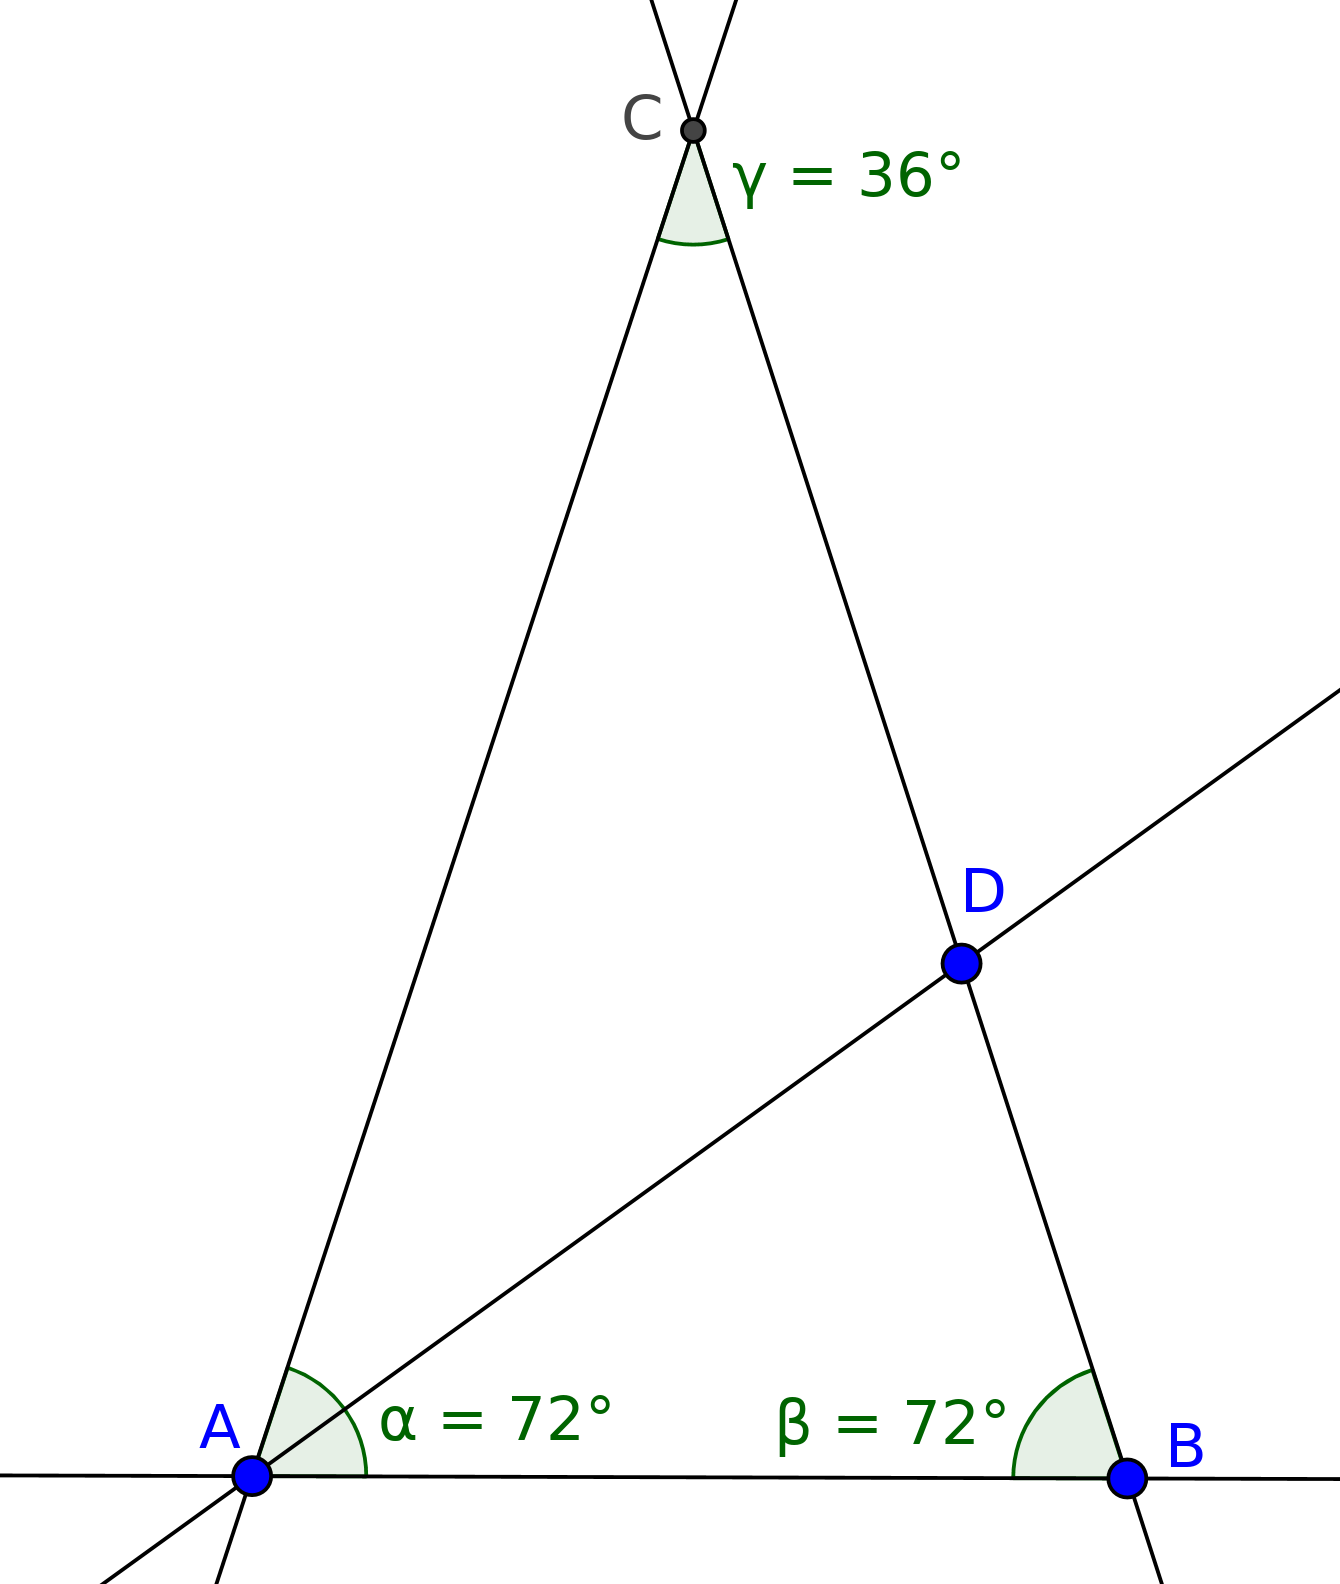
\includegraphics[width=0.3\textwidth]{golden}
            \end{center}
    \begin{parts}
      \part Show that $ ABC $ and $ ABD $ are similar triangles.
      \part Hence, or otherwise, show that $ \frac{AB}{BD} = \frac{AB + BD}{AB} $.
      \part Show that the ratio of the long side of the triangle to the short side
            of the triangle is $ \frac{AB}{BD} = \frac{1 + \sqrt{5}}{2} = \phi $.
      \part Show that $ \cos \ang{72} = \frac{1}{2\phi} $.
      \part Find $ \sin \ang{36} $ and $ \sin \ang{72} $.
    \end{parts}

\end{questions}

\end{document}
